\documentclass[11pt,a4paper,parskip=half ]{scrartcl}
\usepackage[utf8]{inputenc}
\usepackage[ngerman]{babel}
\usepackage{amsfonts}
\usepackage{amssymb}
\usepackage{graphicx}
\usepackage{xcolor}
\usepackage{float}
\usepackage{graphicx}
\usepackage{hyperref}
\usepackage[fleqn]{amsmath}
\usepackage[left=3.00cm, right=3.00cm, top=3.00cm, bottom=3.00cm]{geometry}

\author{Aaron Winziers - 1176638; Michael Wolz - 1195270}
\title{Digital Libraries WS 2018/2019\\\LARGE{Übungsblatt 9}}

\begin{document}
	\maketitle
	
	\section*{Aufgabe 1}
	
	\subsection*{a)}
	 
	\subsubsection*{(Interpolierter) Precision-Recall-Graph}
	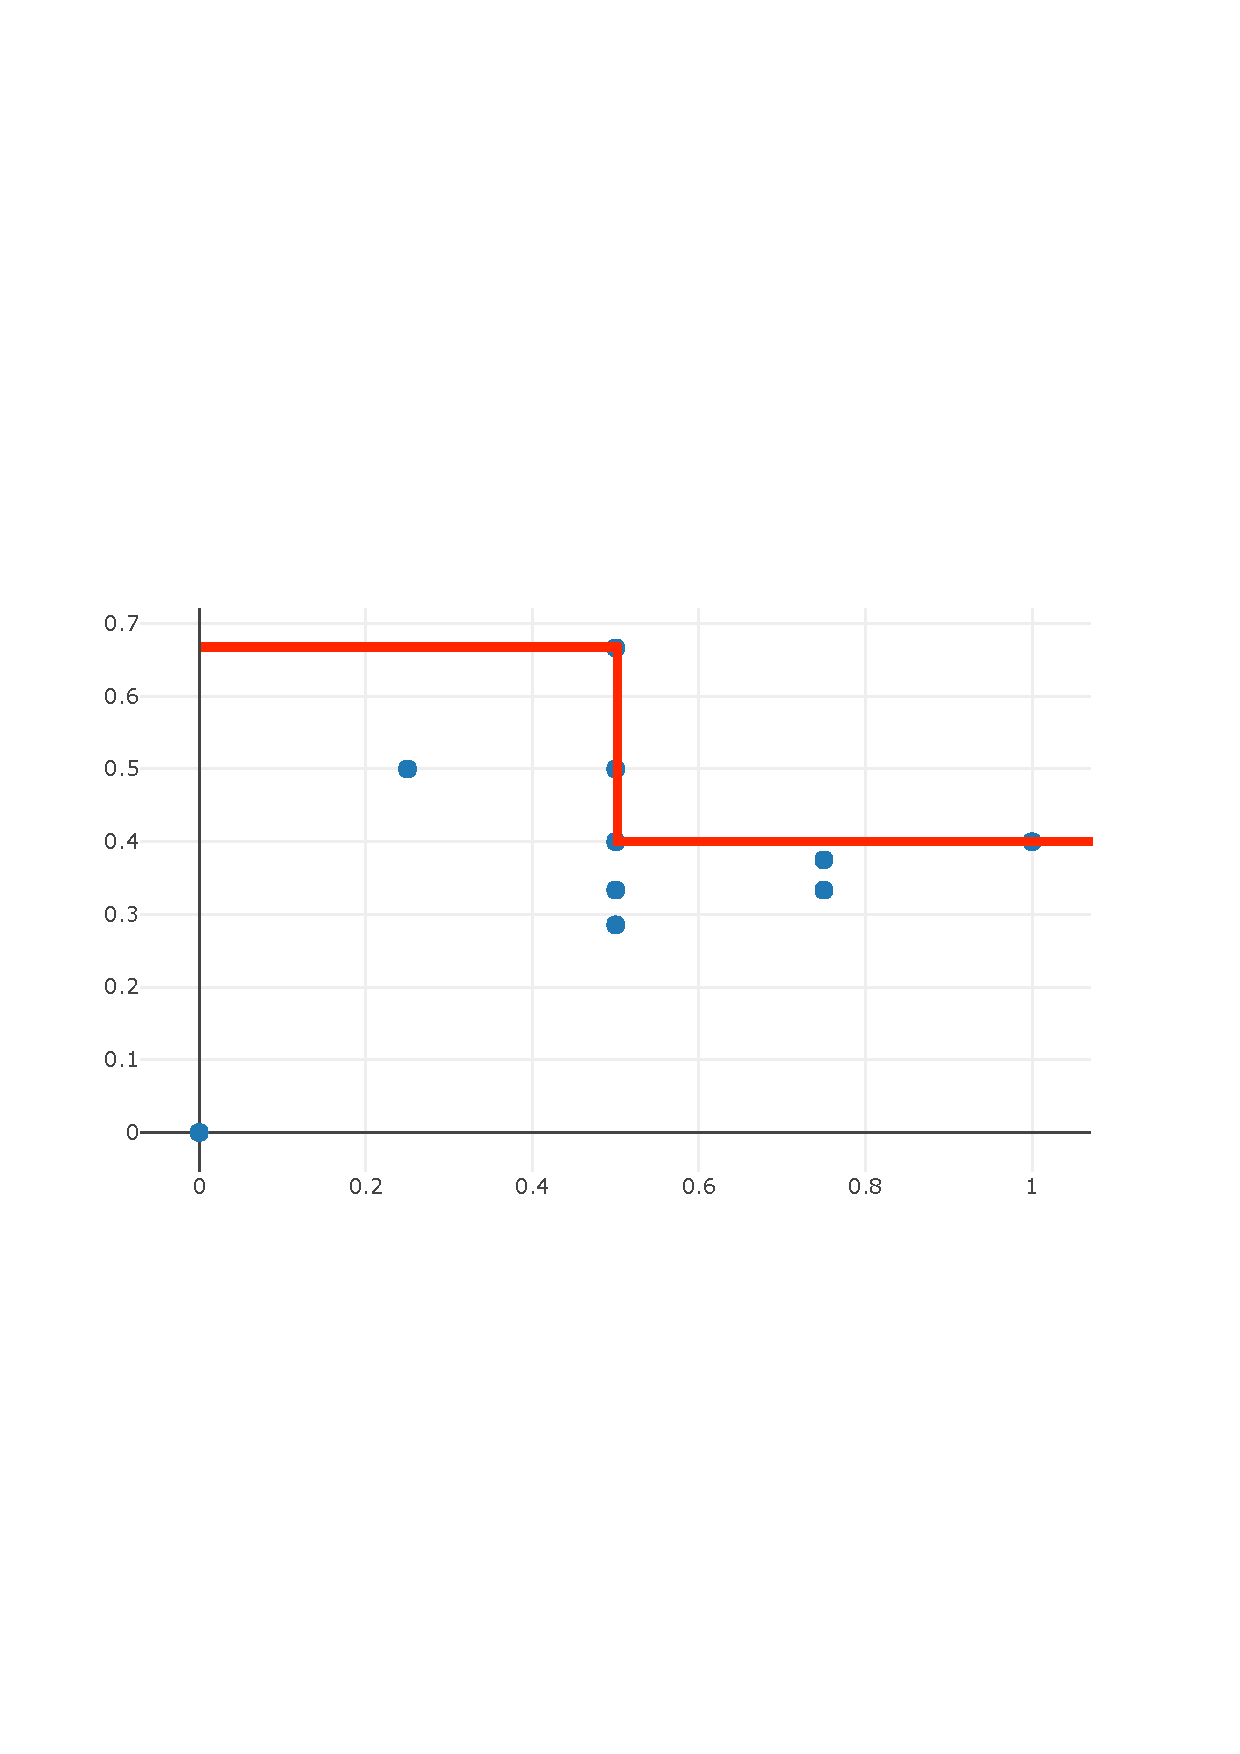
\includegraphics[width=\textwidth]{aufgabe1a.pdf}

	\subsection*{b)}
	
	\begin{table}[H]
		\begin{tabular}{|l|l|l|l|l|l|l|l|l|l|l|l|}
			\hline
			precision & 0.67 & 0.67 & 0.67 & 0.67 & 0.67 & 0.67 & 0.4 & 0.4 & 0.4 & 0.4 & 0.4 \\ \hline
			recall    & 0    & 0.1  & 0.2  & 0.3  & 0.4  & 0.5  & 0.6 & 0.7 & 0.8 & 0.9 & 1   \\ \hline
		\end{tabular}
	\end{table}
	
	$AIP = (0.67 + 0.67 + 0.67 + 0.67 + 0.675 + 0.67 + 0.4 + 0.4 + 0.4 + 0.4 + 0.4) / 11 = 0.55$
	
	\subsection*{c)}
		
	\subsubsection*{1)}
	
	\begin{table}[H]
		\begin{tabular}{|l|l|l|l|l|l|l|l|l|l|l|l|}
			\hline
			precision & 1.0 & 1.0 & 1.0 & 0.5 & 0.5 & 0.5 & 0.5 & 0.5 & 0.4 & 0.4 & 0.4 \\ \hline
			recall    & 0   & 0.1 & 0.2 & 0.3 & 0.4 & 0.5 & 0.6 & 0.7 & 0.8 & 0.9 & 1   \\ \hline
		\end{tabular}
	\end{table}

	\subsubsection*{2)}
	
	\begin{table}[H]
		\begin{tabular}{|l|l|l|l|l|l|l|l|l|l|l|l|}
			\hline
			mean precision & 1.0 & 1.0 & 1.0 & 0.67 & 0.67 & 0.67 & 0.6 & 0.6 & 0   & 0   & 0 \\ \hline
			recall    & 0   & 0.1 & 0.2 & 0.3  & 0.4  & 0.5  & 0.6 & 0.7 & 0.8 & 0.9 & 1 \\ \hline
		\end{tabular}
	\end{table}
	
	
	\subsection*{d)}
	
	\begin{table}[H]
		\begin{tabular}{|l|l|l|l|l|l|l|l|l|l|l|l|}
			\hline
			precision & 0.89 & 0.89 & 0.89 & 0.61 & 0.61 & 0.61 & 0.5 & 0.5 & 0.27 & 0.27 & 0.27 \\ \hline
			recall    & 0    & 0.1  & 0.2  & 0.3  & 0.4  & 0.5  & 0.6 & 0.7 & 0.8  & 0.9  & 1    \\ \hline
		\end{tabular}
	\end{table}

	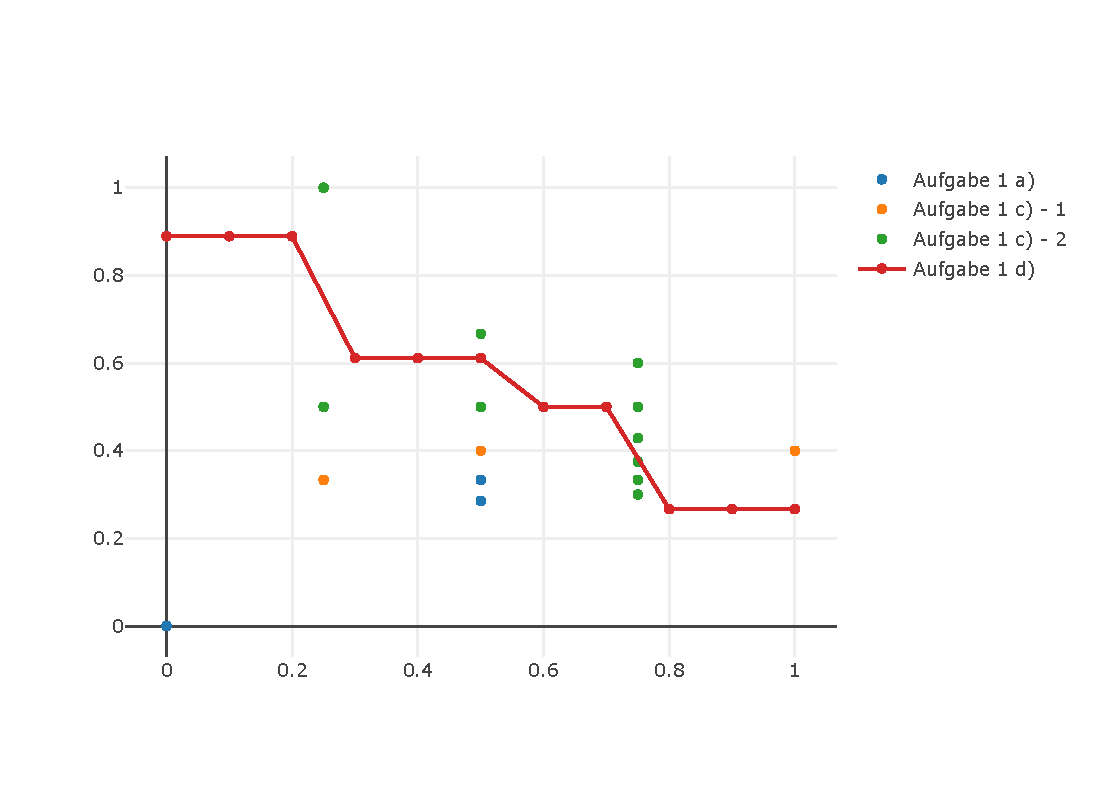
\includegraphics[width=\textwidth]{aufgabe1d.pdf}
	
	
	\section*{Aufgabe 2}
	
	\begin{table}[H]
		\begin{tabular}{|l|l|l|l|l|l|l|l|l|l|l|}
			\hline
			Rang	&	1	&	2	&	3	& 	4	&	5	&	6	&	7	&	8	&	9	&	10	\\
			\hline
			\hline
			Ideal NDCG			&	2	&	4	&	4.63	&	5.13	&	5.13	&	5.13	&	5.13	&	5.13	&	5.13	&	5.13	\\
			\hline
			Aufgabe 1 (NDCG)	&	1.0	&	0.5	&	0.57	&	0.51	&	0.6		&	0.6		&	0.6		&	0.6		&	0.6		&	0.6	\\
			\hline
			Aufgabe 2 (NDCG)	&	1.0	&	0.5	&	0.43	&	0.59	&	0.59	&	0.66	&	0.66	&	0.66	&  0.66 	&  0.72 	\\
			\hline
			Aufgabe 3 (MNDCG)	&	1.0	&	0.5	&	0.5		&	0.55	&	0.59	&	0.63	&	0.63	&	0.63	&	0.63	&	0.66	\\	
			\hline
		\end{tabular}
	\end{table}
	
	
	\section*{Aufgabe 3}
	
	\subsection*{a)}
	
	\subsection*{b)}
	
	\subsection*{c)}
	
	\subsection*{d)}
	
\end{document}